\documentclass[xetex,mathserif,serif]{beamer}
\usepackage{polyglossia}
\setdefaultlanguage[babelshorthands=true]{russian}
\usepackage{minted}
\usepackage{tabu}
\usepackage[11pt]{moresize}

\usepackage{textpos}
\setlength{\TPHorizModule}{1cm}
\setlength{\TPVertModule}{1cm}

\useoutertheme{infolines}

\usepackage{fontspec}
\setmainfont{FreeSans}
\newfontfamily{\russianfonttt}{FreeSans}

\tabulinesep=0.7mm

\newcommand{\attribution}[1] {
    \begin{flushright}\begin{scriptsize}\textcolor{gray}{\textcopyright\; #1}\end{scriptsize}\end{flushright}
}

\title{Лекция 14: Проектирование распределённых приложений}
\subtitle{Часть вторая: стратегические вопросы}
\author[Юрий Литвинов]{Юрий Литвинов\\\small{\textcolor{gray}{y.litvinov@spbu.ru}}}

\date{08.12.2022}

\begin{document}

    \frame{\titlepage}

    \section{Архитектурные стили распределённых систем}

    % Источник: https://github.com/MicrosoftDocs/architecture-center/tree/main/docs/guide/architecture-styles

    \begin{frame}
        \frametitle{Big Compute}
        \begin{center}
            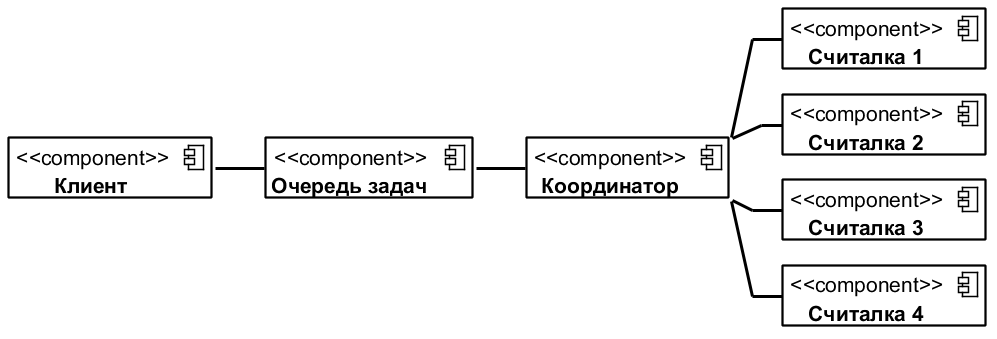
\includegraphics[width=0.8\textwidth]{bigCompute.png}
        \end{center}
        \begin{itemize}
            \item Для сверхсложных задач, предполагающих тысячи вычислительных узлов
            \item Требует <<embarrassingly parallel>> задачу
            \item Предполагает использование весьма продвинутых (и дорогих) облачных ресурсов
        \end{itemize}
    \end{frame}

    \begin{frame}
        \frametitle{Big Data}
        \begin{center}
            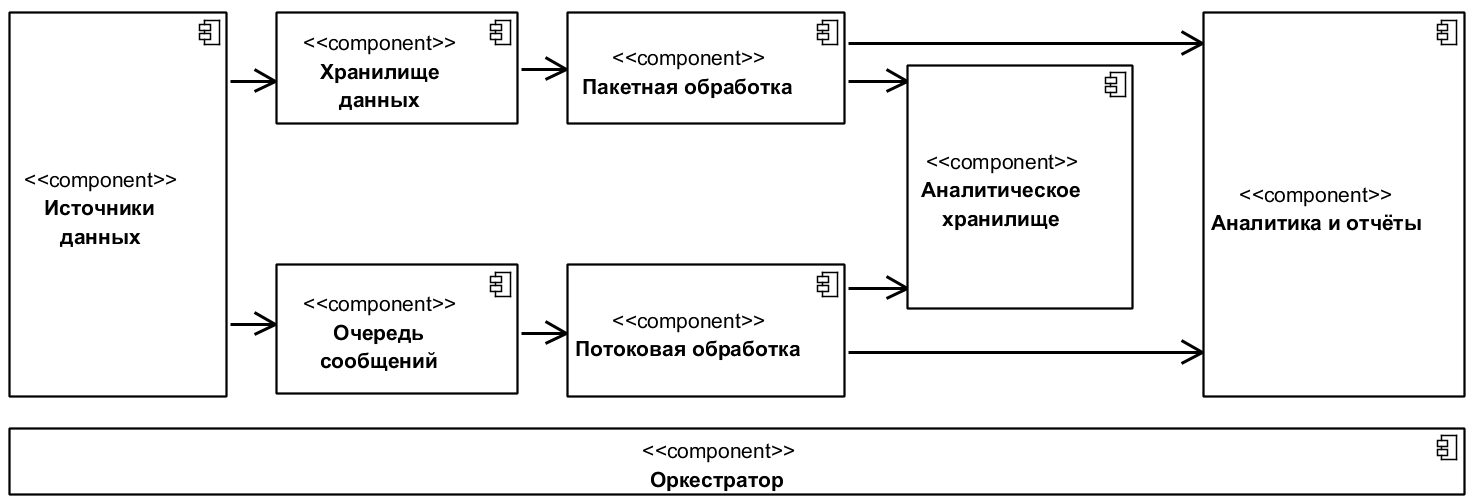
\includegraphics[width=0.9\textwidth]{bigData.png}
        \end{center}
        \begin{itemize}
            \item Для аналитики над большими данными
            \begin{itemize}
                \item Либо данных много и их можно обрабатывать неторопливо
                \item Либо данных много и их надо обрабатывать в реальном времени
            \end{itemize}
            \item Данные не лезут в обычную СУБД
        \end{itemize}
    \end{frame}

    \begin{frame}
        \frametitle{Big Data, хорошие практики}
        \begin{itemize}
            \item Распределённые хранение и обработка
            \begin{itemize}
                \item Например, Apache Hadoop, Apache Spark
            \end{itemize}
            \item Schema-on-read
            \begin{itemize}
                \item Data lake --- распределённое хранилище слабоструктурированных данных
            \end{itemize}
            \item Обработка на месте (TEL вместо ETL)
            \item Разделение данных по интервалам обработки
            \item Раннее удаление приватных данных
        \end{itemize}
    \end{frame}

    \begin{frame}
        \frametitle{Пример: IoT}
        \begin{center}
            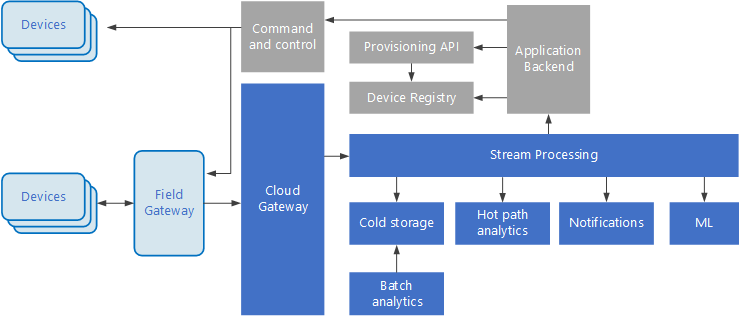
\includegraphics[width=0.9\textwidth]{iot.png}
            \attribution{https://github.com/MicrosoftDocs/architecture-center/blob/main/docs/guide/architecture-styles/big-data.md}
        \end{center}
    \end{frame}

    \begin{frame}
        \frametitle{Событийно-ориентированная архитектура}
        \begin{center}
            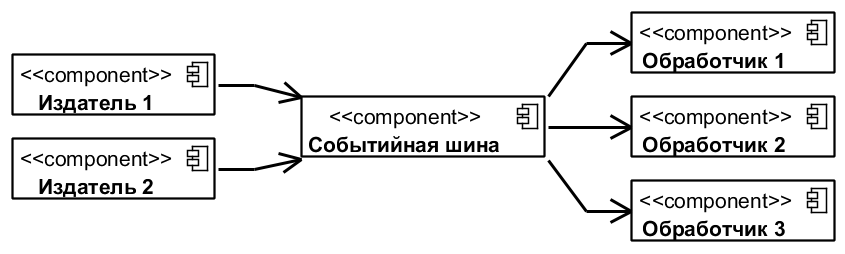
\includegraphics[width=0.7\textwidth]{eventDrivenArchitecture.png}
        \end{center}
        \begin{itemize}
            \item Для обработки событий в реальном времени
            \item Бывает двух видов:
            \begin{itemize}
                \item Издатель/подписчик (например, RabbitMQ)
                \item Event Sourcing (например, Apache Kafka)
            \end{itemize}
        \end{itemize}
    \end{frame}

    \begin{frame}
        \frametitle{Web-queue-worker}
        \begin{center}
            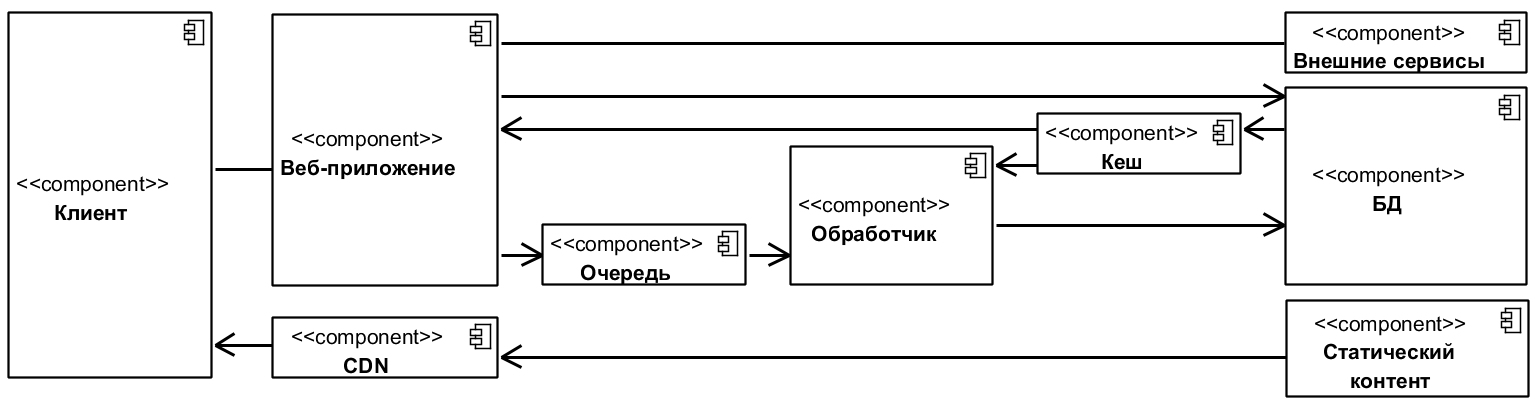
\includegraphics[width=0.9\textwidth]{webQueueWorker.png}
        \end{center}
        \begin{itemize}
            \item Для вычислительно сложных задач в несложной предметной области
            \item Позволяет эффективно использовать готовые сервисы
            \item Независимое масштабирование фронтенда и обработчика
            \item Может превратиться в Big Ball of Mud
        \end{itemize}
    \end{frame}

    \begin{frame}
        \frametitle{N-звенная архитектура}
        \begin{center}
            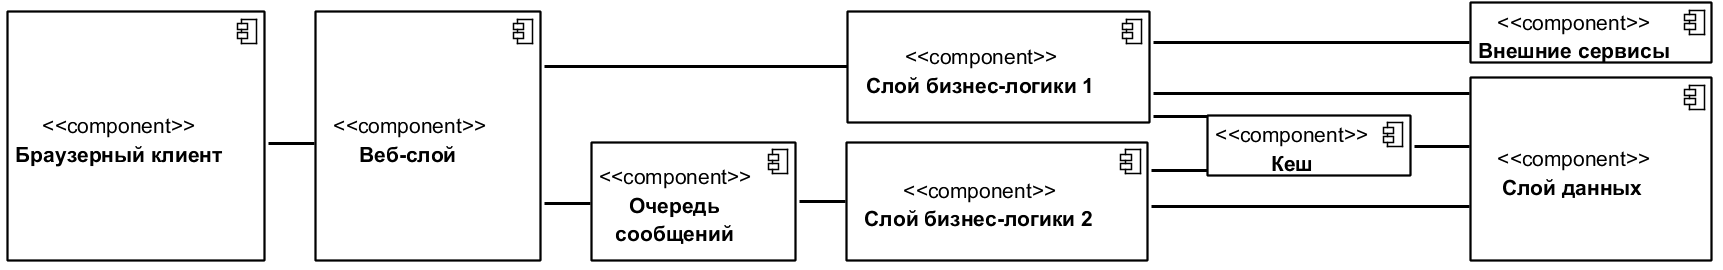
\includegraphics[width=0.9\textwidth]{nTierArchitecture.png}
        \end{center}
        \begin{itemize}
            \item Для быстрого переноса монолита в облако
            \item Для простых веб-приложений
            \item Проблемы с масштабированием и сопровождаемостью
        \end{itemize}
    \end{frame}

    \begin{frame}
        \frametitle{Пример: N-звенное приложение на Azure}
        \begin{center}
            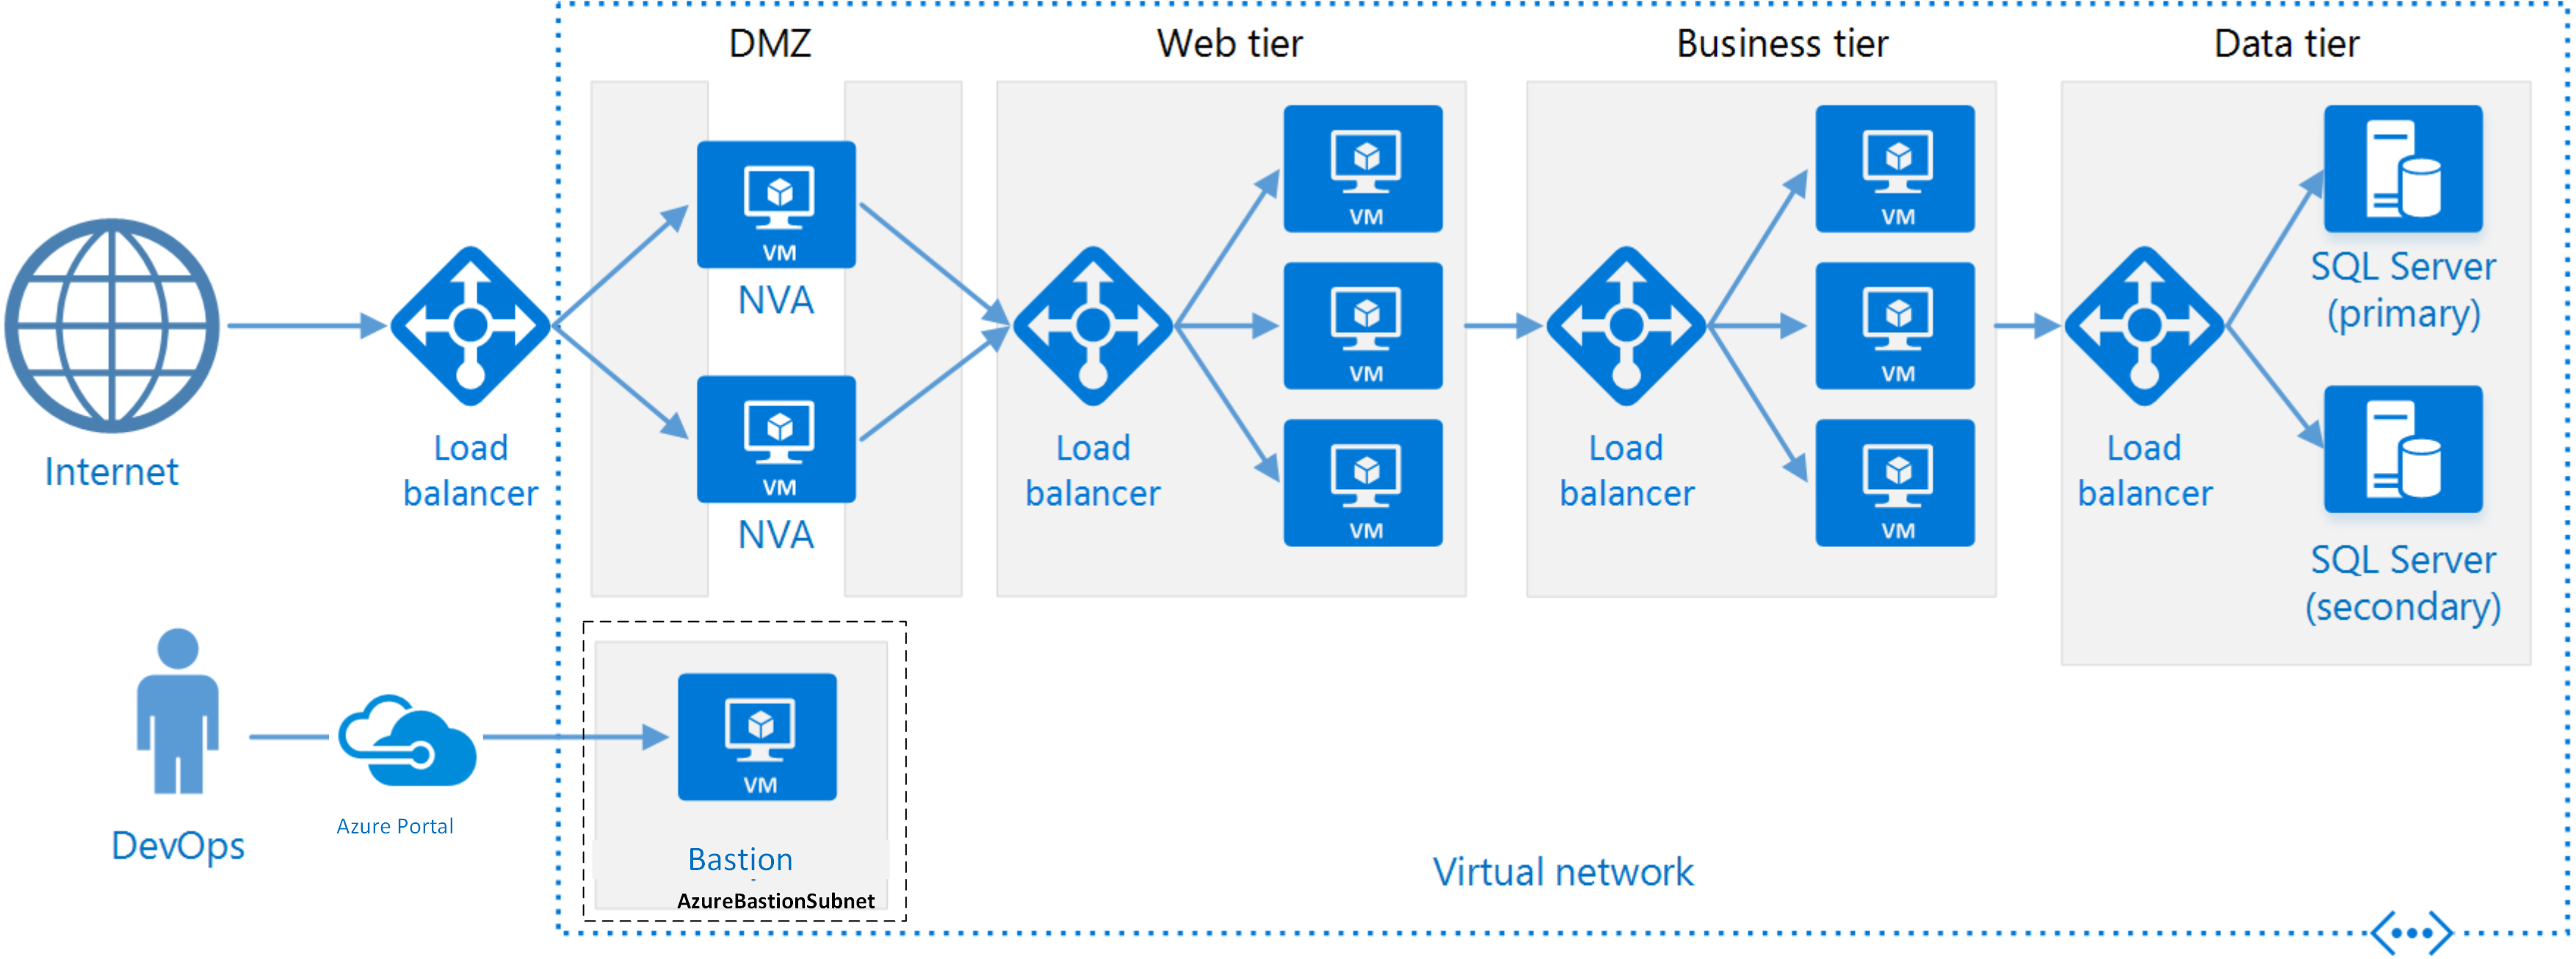
\includegraphics[width=\textwidth]{n-tier-physical-bastion.png}
            \attribution{https://github.com/MicrosoftDocs/architecture-center/blob/main/docs/guide/architecture-styles/n-tier.md}
        \end{center}
    \end{frame}

    \begin{frame}
        \frametitle{Микросервисная архитектура}
        \begin{center}
            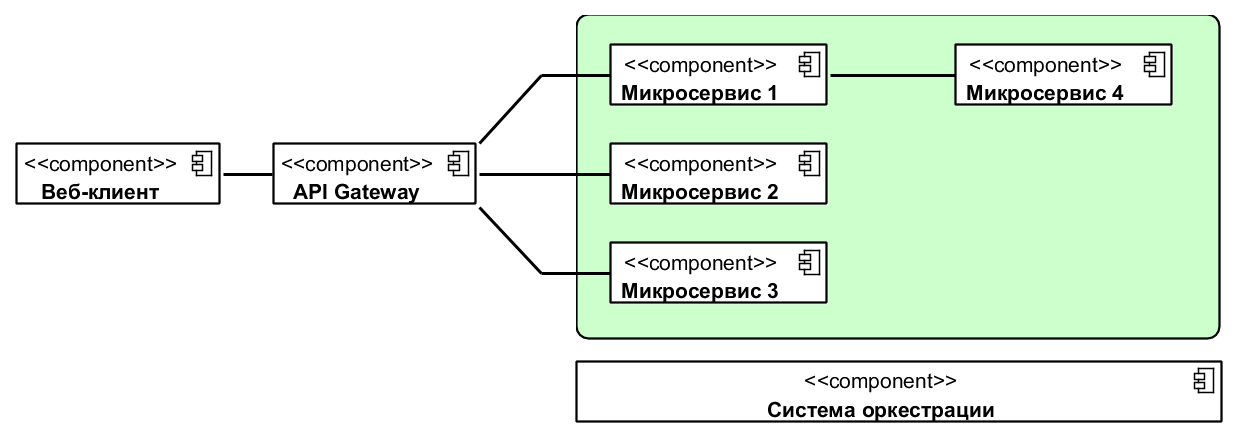
\includegraphics[width=0.85\textwidth]{microservices.png}
        \end{center}
        \begin{itemize}
            \item Для приложений со сложной предметной областью
            \item Альтернатива монолиту, со своими достоинствами и недостатками
            \item Микросервис пишется одним человеком за две недели
            \begin{itemize}
                \item На самом деле, пишется и поддерживается небольшой командой
            \end{itemize}
            \item Микросервис --- ограниченный контекст в смысле DDD
        \end{itemize}
    \end{frame}

    \begin{frame}
        \frametitle{Особенности}
        \begin{itemize}
            \item Каждый микросервис --- отдельное приложение
            \begin{itemize}
                \item Независимость языков и технологий
                \item Имеет своё хранилище данных, не имеет права шарить данные
                \begin{itemize}
                    \item В каком-то смысле, объект из ООП
                    \item Каждому сервису наиболее подходящая СУБД
                \end{itemize}
            \end{itemize}
            \item Мелкозернистая масштабируемость
            \item Независимое развёртывание
            \item Изоляция ошибок
            \item Маленькая и простая кодовая база
        \end{itemize}
    \end{frame}

    \begin{frame}
        \frametitle{Проблемы}
        \begin{itemize}
            \item Сложность перекладывается с реализации на оркестрацию
            \begin{itemize}
                \item Неочевидно, неразвитые инструменты
                \item В целом сложнее, чем рассмотренные выше стили
                \item Сложное управление и мониторинг, требуется развитая культура DevOps
                \item Сложная в плане управления зависимостями разработка
            \end{itemize}
            \item Технологический зоопарк
            \item Нагрузка на сеть
            \item Сложно поддерживать целостность данных
            \begin{itemize}
                \item Eventual Consistency
            \end{itemize}
        \end{itemize}
    \end{frame}

    \section{REST}

    \begin{frame}
        \frametitle{Representational State Transfer (REST)}
        \begin{itemize}
            \item Самая популярная сейчас архитектура веб-сервисов
            \item Передача всего необходимого в запросе
            \begin{itemize}
                \item Нельзя хранить состояние сессии
            \end{itemize}
            \item Стандартизованный интерфейс, очень простые запросы
            \item Стандартные протоколы (в основном поверх HTTP)
            \item Обычно JSON как формат сериализации
            \item Кеширование
        \end{itemize}
    \end{frame}

    \begin{frame}
        \frametitle{Интерфейс сервиса}
        \begin{itemize}
            \item Коллекции
            \begin{itemize}
                \item \url{http://api.example.com/customers/}
            \end{itemize}
            \item Элементы
            \begin{itemize}
                \item \url{http://api.example.com/customers/17}
            \end{itemize}
            \item HTTP-методы (GET, POST, PUT, DELETE), стандартная семантика, стандартные коды ошибок
            \item Передача параметров прямо в URL
            \begin{itemize}
                \item \url{http://api.example.com/customers?user=me&access_token=ASFQF}
            \end{itemize}
        \end{itemize}
    \end{frame}

    \begin{frame}
        \frametitle{Пример, Google Drive REST API}
        \begin{itemize}
            \item GET https://www.googleapis.com/drive/v2/files --- список всех файлов
            \item GET https://www.googleapis.com/drive/v2/files/fileId --- метаданные файла по его Id
            \item POST https://www.googleapis.com/upload/drive/v2/files — загрузить новый файл
            \item PUT https://www.googleapis.com/upload/drive/v2/files/fileId --- обновить файл
            \item DELETE https://www.googleapis.com/drive/v2/files/fileId --- удалить файл
        \end{itemize}
    \end{frame}

    \begin{frame}
        \frametitle{Дизайн REST-интерфейса}
        \begin{itemize}
            \item API строится вокруг ресурсов, не действий
            \begin{itemize}
                \item \url{http://api.example.com/customers/} --- хорошо
                \item \url{http://api.example.com/get_customer/} --- плохо
            \end{itemize}
            \item Отношения между сущностями: \url{http://api.example.com/customers/5/orders}
            \begin{itemize}
                \item Максимум одно отношение --- надо будет, сделают ещё запросы
            \end{itemize}
            \item API --- модель предметной области, не данных
            \item Семантика HTTP
            \begin{itemize}
                \item Заголовки Content-Type, Accept
                \item Коды возврата (200, 204, 404, 400, 409)
            \end{itemize}
            \item Механизмы фильтрации и <<пагинации>>
            \item Поддержка Partial Content
            \item Hypertext as the Engine of Application State (HATEOAS)
            \item Версионирование --- не ломать обратную совместимость
        \end{itemize}
    \end{frame}

    \section{Общие принципы дизайна}

    \begin{frame}
        \frametitle{Общие принципы дизайна распределённых приложений}
        \framesubtitle{Самовосстановление}
        \begin{itemize}
            \item Повтор при временном отказе
            \item Паттерн <<Circuit Breaker>>
            \item API для самодиагностики
            \item Разделение на изолированные группы ресурсов
            \item Буферизация запросов
            \item Автоматическое переключение на резервный экземпляр, ручное обратно
            \item Промежуточное сохранение
            \item Плавная потеря работоспособности (graceful degradation)
            \item Тестирование отказов, Chaos engineering
        \end{itemize}
    \end{frame}

    \begin{frame}
        \frametitle{Избыточность}
        \begin{columns}
            \begin{column}{0.5\textwidth}
                \begin{itemize}
                    \item Бизнес-требования к надёжности
                    \begin{itemize}
                        \item Recovery Time Objective, Recovery Point Objective, Maximum Tolerable Outage
                    \end{itemize}
                    \item Балансировщики нагрузки
                    \item Репликация БД
                    \item Разделение по регионам
                    \item Шардирование
                \end{itemize}
            \end{column}
            \begin{column}{0.5\textwidth}
                \begin{center}
                    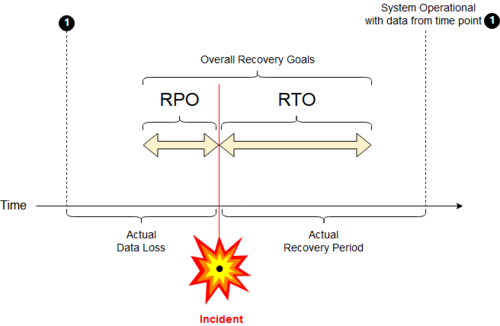
\includegraphics[width=\textwidth]{rpoRtoExample.png}
                    \attribution{\url{https://en.wikipedia.org/wiki/Disaster_recovery}}
                \end{center}
            \end{column}
        \end{columns}
    \end{frame}

    \begin{frame}
        \frametitle{Минимизация координации}
        \begin{itemize}
            \item Доменные события (domain events)
            \item Паттерн <<Command and Query Responsibility Segregation>> (CQRS)
            \item Event Sourcing
            \item Асинхронные, идемпотентные операции
            \item Шардирование
            \item Eventual Consistency, компенсационные транзакции
        \end{itemize}
    \end{frame}

    \begin{frame}
        \frametitle{CAP-теорема}
        В любой распределённой системе можно обеспечить не более двух из трёх свойств:
        \begin{itemize}
            \item Согласованность данных (Consistency) --- во всех вычислительных узлах данные консистентны
            \item Доступность (Availability) --- любой запрос завершается корректно, но без гарантии, что ответы всех узлов одинаковы
            \item Устойчивость к разделению (Partitioning Tolerance) --- потеря связи между узлами не портит ответы
            \begin{itemize}
                \item Этот пункт в распределённых системах должен быть обеспечен всегда, потому что отказы неизбежны. Остаётся выбрать один из двух
            \end{itemize}
        \end{itemize}
    \end{frame}

    \begin{frame}
        \frametitle{ACID vs BASE}
        ACID:
        \begin{itemize}
            \item Atomicity --- транзакция не применится частично
            \item Consistency --- завершённая транзакция не нарушает целостности данных
            \item Isolation --- параллельные транзакции не мешают друг другу
            \item Durability --- если транзакция завершилась, её данные не потеряются
        \end{itemize}
        BASE:
        \begin{itemize}
            \item Basically Available --- отказ узла может привести к некорректному ответу, но только для клиентов, обслуживавшихся узлом
            \item Soft-state --- состояние может меняться само собой, согласованность между узлами не гарантируется
            \item Eventually consistent --- гарантируется целостность только в некоторый момент в будущем
        \end{itemize}
    \end{frame}

    \begin{frame}
        \frametitle{Проектирование для обслуживания}
        \begin{itemize}
            \item Делать всё наблюдаемым
            \begin{itemize}
                \item Трассировка, в т.ч. распределённая
                \item Логирование 
            \end{itemize}
            \item Мониторинг, метрики
            \item Стандартизация форматов логов и метрик
            \item Автоматизация задач обслуживания
            \item Конфигурация --- это код
        \end{itemize}
    \end{frame}

    \section{Docker}

    \begin{frame}
        \frametitle{Docker}
        \begin{itemize}
            \item Средство для ``упаковки'' приложений в изолированные контейнеры
            \item Что-то вроде легковесной виртуальной машины
            \item Широкий инструментарий: DSL для описания образов, публичный репозиторий, поддержка оркестраторами
        \end{itemize}
        \begin{center}
            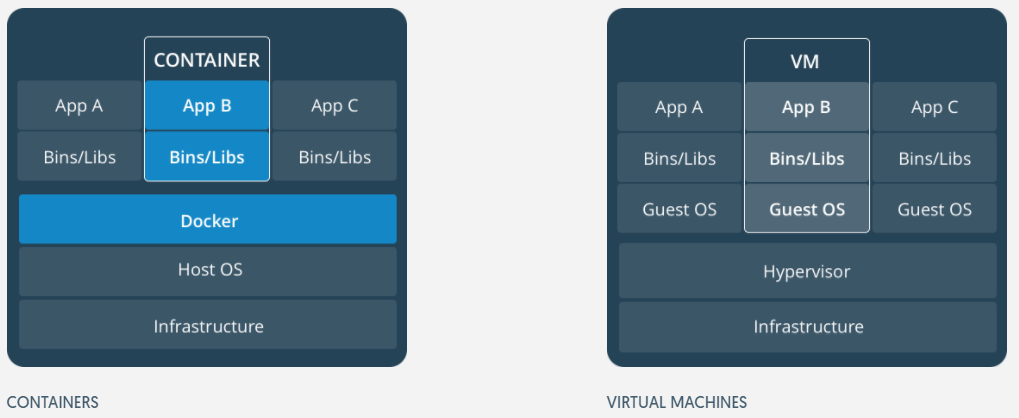
\includegraphics[width=0.7\textwidth]{docker.png}
            \attribution{\url{https://www.docker.com}}
        \end{center}
    \end{frame}

    \begin{frame}
        \frametitle{Docker Image}
        \begin{columns}
            \begin{column}{0.6\textwidth}
                \begin{itemize}
                    \item Окружение и приложение
                    \item Состоит из слоёв
                    \begin{itemize}
                        \item Все слои read-only
                        \item Образы делят слои между собой как процессы делят динамические библиотеки
                    \end{itemize}
                    \item На основе одного образа можно создать другой
                \end{itemize}
            \end{column}
            \begin{column}{0.4\textwidth}
                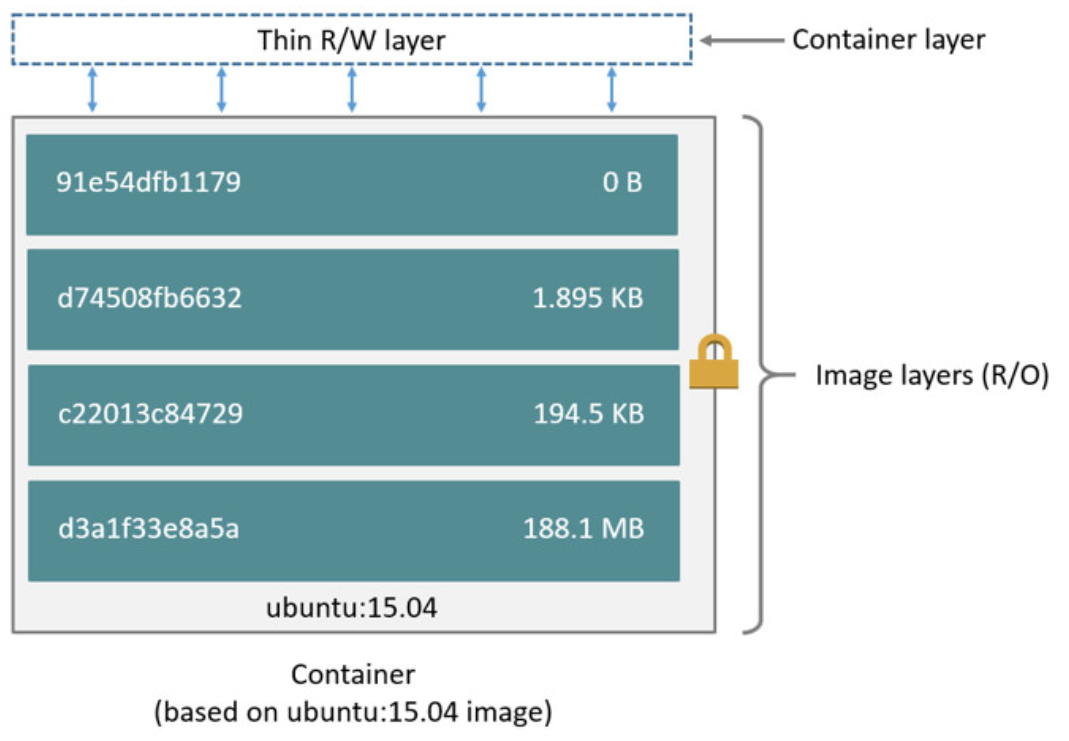
\includegraphics[width=0.9\textwidth]{dockerLayers.png}
            \end{column}
        \end{columns}
    \end{frame}

    \begin{frame}
        \frametitle{Docker Container}
        \begin{columns}
            \begin{column}{0.5\textwidth}
                \begin{itemize}
                    \item Образ с дополнительным write слоем
                    \item Содержит один запущенный процесс
                    \item Может быть сохранен как новый образ
                \end{itemize}
            \end{column}
            \begin{column}{0.5\textwidth}
                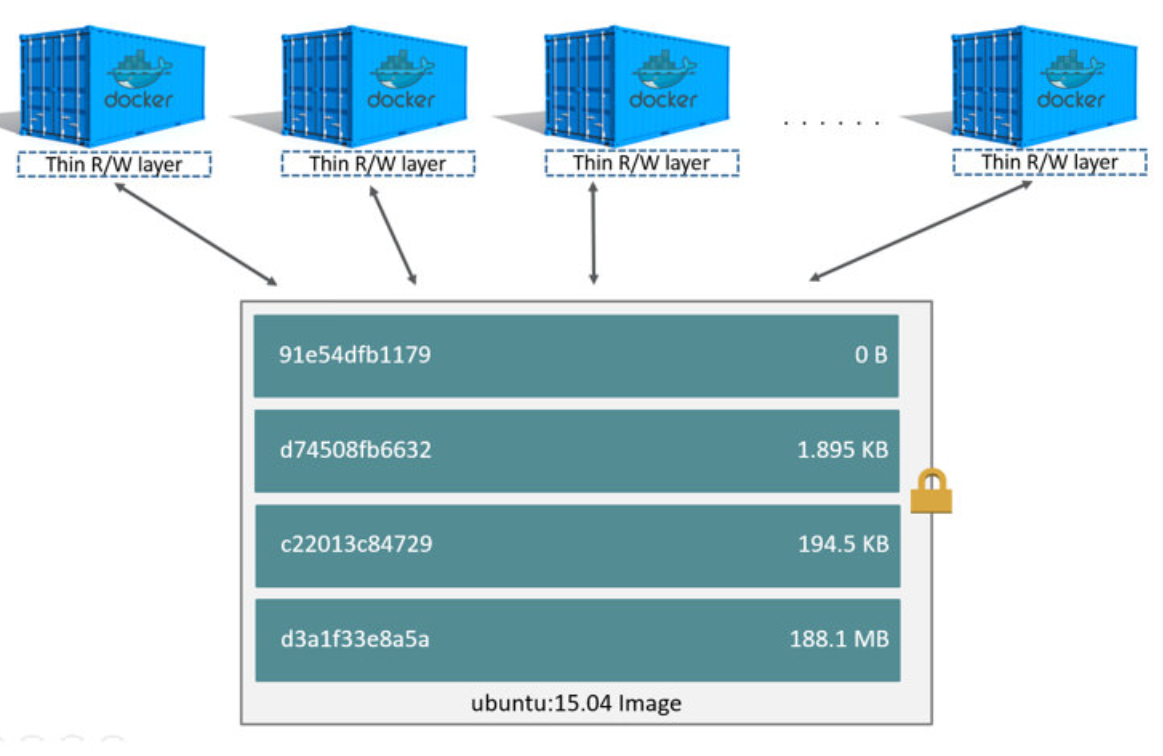
\includegraphics[width=0.9\textwidth]{dockerContainer.png}
            \end{column}
        \end{columns}
    \end{frame}

    \begin{frame}
        \frametitle{DockerHub}
        \begin{columns}
            \begin{column}{0.5\textwidth}
                \begin{itemize}
                    \item Внешний репозиторий образов
                    \begin{itemize}
                        \item Официальные образы
                        \item Пользовательские образы
                        \item Приватные репозитории
                    \end{itemize}
                    \item Простой CI/CD
                    \item Высокая доступность
                \end{itemize}
            \end{column}
            \begin{column}{0.5\textwidth}
                
\includegraphics[width=0.9\textwidth]{dockerHub.png}
            \end{column}
        \end{columns}
    \end{frame}

    \begin{frame}
        \frametitle{Базовые команды}
        \begin{itemize}
            \item docker run --- запускает контейнер (при необходимости делает pull)
            \begin{itemize}
                \item -d --- запустить в фоновом режиме
                \item -p host\_port:container\_port --- прокинуть порт из контейнера на хост
                \item -i -t --- запустить в интерактивном режиме
                \item Пример: \mintinline{text}|docker run -it ubuntu /bin/bash|
            \end{itemize}
            \item docker ps --- показывает запущенные контейнеры
            \begin{itemize}
                \item Пример: \mintinline{text}|docker run -d nginx; docker ps|
            \end{itemize}
            \item docker stop --- останавливает контейнер (шлёт SIGTERM, затем SIGKILL)
            \item docker exec --- запускает дополнительный процесс в контейнере
        \end{itemize}
    \end{frame}

    \begin{frame}[fragile]
        \frametitle{Dockerfile}
        \begin{scriptsize}
            \begin{minted}{sh}
# Use an official Python runtime as a parent image
FROM python:2.7-slim

# Set the working directory to /app
WORKDIR /app

# Copy the current directory contents into the container at /app
ADD . /app

# Install any needed packages specified in requirements.txt
RUN pip install --trusted-host pypi.python.org -r requirements.txt

# Make port 80 available to the world outside this container
EXPOSE 80

# Define environment variable
ENV NAME World

# Run app.py when the container launches
CMD ["python", "app.py"]
            \end{minted}
        \end{scriptsize}
    \end{frame}

    \begin{frame}[fragile]
        \frametitle{Двухфазная сборка}
        \begin{scriptsize}
            \begin{minted}{html}
FROM mcr.microsoft.com/dotnet/aspnet:6.0 AS base
WORKDIR /app
EXPOSE 80
EXPOSE 443

FROM mcr.microsoft.com/dotnet/sdk:6.0 AS build
WORKDIR /src
COPY ["ConferenceRegistration/ConferenceRegistration.csproj", "ConferenceRegistration/"]
RUN dotnet restore "ConferenceRegistration/ConferenceRegistration.csproj"
COPY . .
WORKDIR "/src/ConferenceRegistration"
RUN dotnet build "ConferenceRegistration.csproj" -c Release -o /app/build

FROM build AS publish
RUN dotnet publish "ConferenceRegistration.csproj" -c Release -o /app/publish

FROM base AS final
WORKDIR /app
COPY --from=publish /app/publish .
ENTRYPOINT ["dotnet", "ConferenceRegistration.dll"]
            \end{minted}
        \end{scriptsize}
    \end{frame}

    \begin{frame}[fragile]
        \frametitle{Docker Compose}
        \begin{scriptsize}
            \begin{minted}{yaml}
version: "3"
services:
    web:
        image: username/repo:tag
        deploy:
            replicas: 5
            resources:
                limits:
                    cpus: "0.1"
                    memory: 50M
            restart_policy:
                condition: on-failure
        ports:
            - "80:80"
        networks:
            - webnet
networks:
    webnet:
            \end{minted}
        \end{scriptsize}
    \end{frame}

    \begin{frame}
        \frametitle{Docker Swarm}
        \begin{itemize}
            \item Машина, на которой запускается контейнер, становится главной
            \item Другие машины могут присоединяться к swarm-у и получать копию контейнера
            \item Docker балансирует нагрузку по машинам
        \end{itemize}
        \begin{center}
            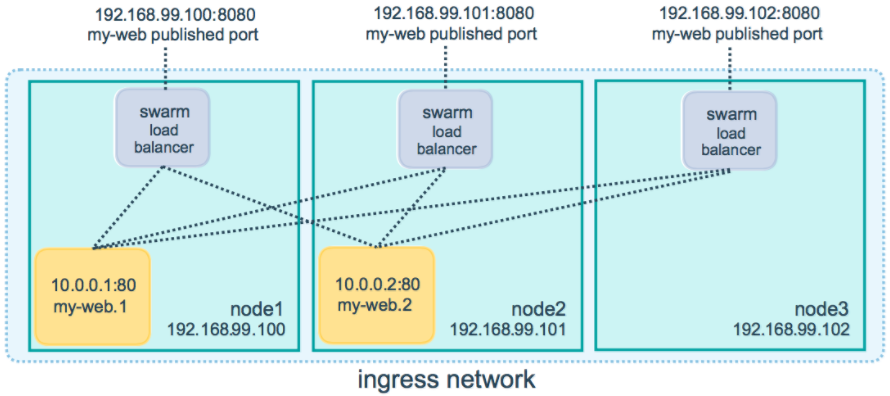
\includegraphics[width=0.7\textwidth]{swarmLoadBalancing.png}
            \attribution{\url{https://www.docker.com}}
        \end{center}
    \end{frame}

    \section{Kubernetes}

    % Источник: Cloud Native DevOps with Kubernetes

    \begin{frame}
        \frametitle{Kubernetes}
        \begin{itemize}
            \item Оркестратор контейнеров
            \item Отвечает за раскидывание контейнеров по хостам, масштабирование, мониторинг и управление жизненным циклом
            \begin{itemize}
                \item Сильно продвинутый Docker Compose
            \end{itemize}
            \item Open-source, Google, Go
        \end{itemize}
        \begin{flushright}
            
\includegraphics[width=0.2\textwidth]{kubernetes.png}
            \hspace{1cm}
            \attribution{\url{https://kubernetes.io/}}
        \end{flushright}
    \end{frame}

    \begin{frame}
        \frametitle{Архитектура Kubernetes}
        \begin{center}
            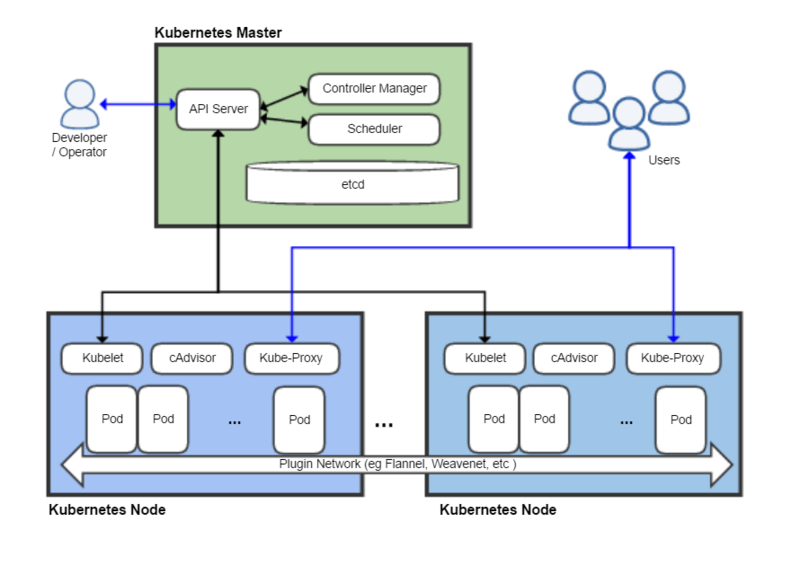
\includegraphics[width=0.8\textwidth]{kubernetesArchitecture.png}
            \attribution{\url{https://ru.wikipedia.org/wiki/Kubernetes}}
        \end{center}
    \end{frame}

    \begin{frame}
        \frametitle{Объекты Kubernetes}
        \begin{center}
            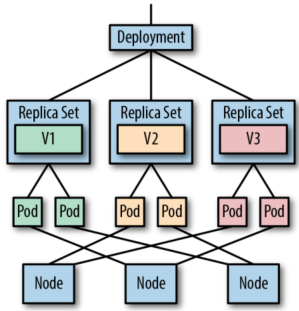
\includegraphics[width=0.4\textwidth]{kubernetesObjects.png}
            \attribution{J. Arundel, J. Domingus, Cloud Native DevOps with Kubernetes}
        \end{center}
    \end{frame}

    \begin{frame}[fragile]
        \frametitle{Deployment}
        \begin{columns}
            \begin{column}{0.5\textwidth}
                \begin{scriptsize}
                    \begin{minted}{yaml}
apiVersion: apps/v1
kind: Deployment
metadata:
  name: demo
  labels:
    app: demo
spec:
  replicas: 1
  selector:
    matchLabels:
      app: demo
  template:
    metadata:
      labels:
        app: demo
    spec:
      containers:
        - name: demo
          image: cloudnatived/demo:hello
          ports:
          - containerPort: 8888
                    \end{minted}
                \end{scriptsize}
            \end{column}
            \begin{column}{0.5\textwidth}
                Запуск:
                \begin{minted}{text}
kubectl apply -f k8s/deployment.yaml
                \end{minted}
                \attribution{J. Arundel, J. Domingus, Cloud Native DevOps with Kubernetes}
            \end{column}
        \end{columns}
    \end{frame}

    \begin{frame}
        \frametitle{Сервисы}
        \begin{center}
            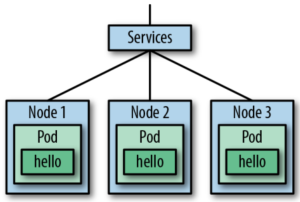
\includegraphics[width=0.4\textwidth]{kubernetesServices.png}
            \attribution{J. Arundel, J. Domingus, Cloud Native DevOps with Kubernetes}
        \end{center}
    \end{frame}

    \begin{frame}[fragile]
        \frametitle{Service}
        \begin{footnotesize}
            \begin{minted}{yaml}
apiVersion: v1
kind: Service
metadata:
  name: demo
  labels:
    app: demo
spec:
  ports:
  - port: 9999
    protocol: TCP
    targetPort: 8888
  selector:
    app: demo
  type: ClusterIP
            \end{minted}
        \end{footnotesize}
        Запуск:
        \begin{minted}{text}
            kubectl apply -f k8s/service.yaml
            kubectl port-forward service/demo 9999:8888
        \end{minted}
        \attribution{J. Arundel, J. Domingus, Cloud Native DevOps with Kubernetes}
    \end{frame}

    \begin{frame}[fragile]
        \frametitle{Рекомендации и техники}
        \begin{itemize}
            \item Конфигурация --- это код, не управляйте кластером вручную
            \item Мониторинг
                \begin{scriptsize}
                    \begin{minted}{yaml}
livenessProbe:
    httpGet:
        path: /healthz
        port: 8888
    initialDelaySeconds: 3
    periodSeconds: 3
                    \end{minted}
                \end{scriptsize}
            \item Blue/green deployment, rainbow deployment, canary deployment
            \begin{itemize}
                \item Не используйте тэг latest для Docker-образов
            \end{itemize}
            \item Используйте инструменты
            \begin{itemize}
                \item Helm, Kubernetes Dashboard и аналоги, Prometheus, Clair, Velero, ...
            \end{itemize}
            \item Метрики: Requests-Errors-Duration, Utilization-Saturation-Errors
        \end{itemize}
    \end{frame}

    \section{Облачная инфраструктура}

    \begin{frame}
        \frametitle{Облачная инфраструктура}
        \begin{itemize}
            \item Виды сервисов:
            \begin{itemize}
                \item Infrastructure as a Service
                \item Platform as a Service
                \item Software as a Service
            \end{itemize}
            \item Основные провайдеры:
            \begin{itemize}
                \item Amazon Web Services (почти 50\% рынка)
                \item Microsoft Azure (порядка 10\%)
                \item Google Cloud
                \item Всё остальное (Heroku, Yandex.Cloud, ...)
            \end{itemize}
        \end{itemize}
    \end{frame}

    % Источник: https://docs.google.com/presentation/d/13pCPuvsjATqodW5iN1qVkIU0_BEz4lYhAKTp6TbWMA0 (с разрешения Владислава Танкова)

    \begin{frame}
        \frametitle{Пример: экосистема AWS}
        \begin{itemize}
            \item Вычисления:
            \begin{itemize}
                \item EC2 (Elastic Computations)
                \item ECS (Elastic Container Service)
            \end{itemize}
            \item Сеть:
            \begin{itemize}
                \item VPC (Virtual Private Cloud)
                \item ELB (Elastic Load Balancer)
                \item API Gateway
            \end{itemize}
            \item Устройства хранения:
            \begin{itemize}
                \item EFS (Elastic File System)
                \item EBS (Elastic Block Storage)
            \end{itemize}
            \item SaaS, базы данных:
            \begin{itemize}
                \item RDS (Relational Database Service)
                \item DynamoDB
                \item ElasticSearch Service
            \end{itemize}
        \end{itemize}
    \end{frame}

    \begin{frame}
        \frametitle{Infrastructure as Code}
        \begin{columns}
            \begin{column}{0.7\textwidth}
                <<The enabling idea of infrastructure as a code is that systems and devices which are used to run software can be treated as if they, themselves, are software>> (Infrastructure as Code, Kief Morris)
                \begin{itemize}
                    \item Платформонезависимое представление инфраструктуры
                    \item Воспроизводимое развёртывание
                    \item Пример: Terraform
                \end{itemize}
            \end{column}
            \begin{column}{0.3\textwidth}
                \begin{center}
                    
\includegraphics[width=0.9\textwidth]{terraformLogo.png}
                \end{center}
            \end{column}
        \end{columns}
    \end{frame}

\end{document}
